\documentclass[12pt,handout]{beamer}

%\documentclass{beamer}
\usetheme{Boadilla}
\useoutertheme{split}
\usepackage{fancyvrb}
\usepackage{tikz}
\usepackage{svg}
\usetikzlibrary{shapes, calc, shapes, arrows, datavisualization}

\usepackage{amsmath,amssymb}

\definecolor{myblue}{RGB}{80,80,160}
\definecolor{exerciseblue}{RGB}{200, 200, 247}
\definecolor{mygreen}{RGB}{80,160,80}


\title{Integer Programming}
\author{Abr\'emod Training}
\titlegraphic{
\includegraphics[scale=0.1]{abremodlogo.png}}

\begin{document}
\setbeamertemplate{caption}{\insertcaption}

\begin{frame}
\titlepage
\end{frame}

\begin{frame}
\frametitle{Integer Programming (IP)}
\begin{itemize}
\item Linear Programming Axioms
\begin{itemize}
\item Additivity
\item Proportionality
\item {\color{red} Divisibility}
\item Certainty
\end{itemize}
\item Fractional solutions are not always suitable
\item Binary decision variables greatly enrich our modeling capability
\end{itemize}
\end{frame}

\begin{frame}
\frametitle{Integer Programming (IP)}
\begin{eqnarray}
z^* = \min / \max && c_1 x_1 + c_2 x_2 + \cdots + c_n x_n \nonumber \\
\mbox{subject to:} &&a_{i1} x_1 + a_{i2} x_2 + \cdots + a_{in} x_n
\begin{Bmatrix}   \le \\
                   \ge \\
                    =
\end{Bmatrix}
b_i,\;\;i = 1,\ldots,m \nonumber \\
&&0 \le x_j \le u_j,\;\;j = 1,\ldots,n \nonumber \\
&&x_j \;\;\mbox{integer for some or all}\;\; j = 1,\ldots,n \nonumber
\end{eqnarray}
\end{frame}

\begin{frame}
\frametitle{Transportation Problem, Revisited}
\begin{itemize}
\item Sets and Indices
    \begin{itemize}
    \item $i \in I$: warehouses
    \item $j \in J$: demand centers (customers)
    \end{itemize}
\item Data
    \begin{itemize}
    \item $u_i$: capacity for warehouse $i$ (widgets)
    \item $d_j$: demand at demand center $j$ (widgets)
    \item $c_{ij}$: shipping cost from warehouse $i$ to demand center $j$ (\$/widget)
    \end{itemize}
\item Decision Variables
    \begin{itemize}
    \item $x_{ij}$: number of widgets to ship from warehouse $i$ to demand center $j$
    \end{itemize}
\end{itemize}
\end{frame}

\begin{frame}
\frametitle{Transportation Problem, Revisited}
\begin{eqnarray}
\min_{x} && \sum_{i \in I} \sum_{j \in J} c_{ij} x_{ij} \;\; \mbox{(minimize shipping costs)} \nonumber \\
\mbox{s.t.} && \sum_{i \in I} x_{ij} = d_j,\;\;j \in J \;\; \mbox{(satisfy demand)}\nonumber \\
&& \sum_{j \in J} x_{ij} \le u_i,\;\;i \in I \;\; \mbox{(don't exceed capacity)} \nonumber \\
&& x_{ij} \ge 0, \;\;i \in I,\;j \in J \;\; \mbox{(ship nonnegative quantities)} \nonumber
\end{eqnarray}
\end{frame}

\begin{frame}
\frametitle{Transportation Problem Extensions}
\begin{itemize}
\item No more than half of customer 3's deliveries come from warehouses 1, 2, and 27 (LP)
\item No more than half the warehouses can be built (IP)
\item Each customer is served by a single warehouse (IP)
\item Allow for unsatisfied demand, at a penalty
    \begin{itemize}
    \item per unit shortage penalty (LP)
    \item increasing unit penalties above threshold values (LP)
    \end{itemize}
\end{itemize}
\end{frame}

\begin{frame}
\frametitle{Transportation Problem Extensions}
\begin{itemize}
\item Increasing marginal shipping costs
    \begin{itemize}
    \item shipping cost $(i,j)$ is $c_{ij} x_{ij}^2$ (easy nonlinear program)
    \item marginal shipping cost is $c_{ij}$ for $0 \le x_{ij} \le l_{ij}$ and $1.5c_{ij}$ for $x_{ij} > l_{ij}$ (LP)
    \end{itemize}
\item Decreasing marginal shipping costs (bulk discounts or economies of scale)
    \begin{itemize}
    \item shipping cost $(i,j)$ is $c_{ij} \sqrt{x_{ij}}$ (difficult nonlinear program)
    \item marginal shipping cost is $c_{ij}$ for $0 \le x_{ij} \le l_{ij}$ and $0.75c_{ij}$ for $x_{ij} > l_{ij}$ (IP)
    \end{itemize}
\item Fixed-charge to open a warehouse (IP)
\end{itemize}
\end{frame}


\begin{frame}
\frametitle{Transportation Problem Extensions}
\begin{itemize}
\item No more than 10 warehouses built
\begin{equation}
\sum_{i \in I} y_i \le 10 \nonumber
\end{equation}
\item Build at most one warehouse at locations $i = 1,13,101$
\begin{equation}
y_1 + y_{13} + y_{101} \le 1 \nonumber
\end{equation}
\item A customer can receive widgets from only one warehouse. Let $w_{ij} = 1$ if customer $j$ receives widgets from warehouse $i$, 0 otherwise
\begin{eqnarray}
&& \sum_{i \in I} w_{ij} = 1,\;\;j \in J \nonumber \\
&& x_{ij} \le d_j w_{ij},\;\;i \in I,\;j \in J \nonumber \\
&& w_{ij} \in \{0,1\},\;\;i \in I,\;j \in J \nonumber
\end{eqnarray}
\end{itemize}
\end{frame}

\begin{frame}
\frametitle{Transportation Problem Extensions}
\begin{itemize}
\item Marginal shipping cost is $c_{ij}$ for $0 \le x_{ij} \le l_{ij}$ and $0.75c_{ij}$ for $x_{ij} > l_{ij}$ \\
$z_{ij}$ indicates whether we ship at least $l_{ij}$ widgets from $i$ to $j$ \\
$x_{ij}^1$ and $x_{ij}^2$ are shipping volumes at level 1 and at level 2
\begin{eqnarray}
\min_{x,z} && \sum_{i \in I} \sum_{j \in J} (c_{ij} x_{ij}^1 + 0.75 c_{ij} x_{ij}^2) \nonumber \\
\mbox{s.t.} && l_{ij} z_{ij} \le x_{ij}^1 \le l_{ij},\;\;i \in I,\;j \in J \nonumber \\
&& 0 \le x_{ij}^2 \le (d_j - l_{ij}) z_{ij},\;\;i \in I,\;j \in J \nonumber \\
&& \sum_{j \in J} (x_{ij}^1 + x_{ij}^2) \le u_i,\;\;i \in I \nonumber \\
&& \sum_{i \in I} (x_{ij}^1 + x_{ij}^2) = d_j,\;\;j \in J \nonumber \\
&& z_{ij} \in \{0,1\},\;\;i \in I,\;j \in J \nonumber \\
&& ... \nonumber
\end{eqnarray}
\end{itemize}
\end{frame}

\begin{frame}
\frametitle{Transportation Problem with Fixed Costs}
Let $f_i$ be the cost of opening a warehouse and $y_i$ indicate whether we open warehouse $i$.
\begin{eqnarray}
\min_{x} && \sum_{i \in I} \sum_{j \in J} c_{ij} x_{ij} + {\color{red} \sum_{i \in I} f_i y_i} \nonumber \\
\mbox{s.t.} && \sum_{i \in I} x_{ij} = d_j,\;\;j \in J \nonumber \\
&& \sum_{j \in J} x_{ij} \le {\color{red} u_i y_i},\;\;i \in I \nonumber \\
&& x_{ij} \ge 0, \;\;i \in I,\;j \in J \nonumber \\
&& {\color{red} y_i \in \{0, 1\},\;\;i \in I} \nonumber
\end{eqnarray}
\end{frame}

{
\setbeamercolor{background canvas}{bg=exerciseblue}
\begin{frame}
\frametitle{Exercise}
Extend the transportation problem to include a fixed costs for opening warehouses. (Set vtype = GRB.BINARY for the new decision variables).
\end{frame}
}

\begin{frame}
\frametitle{How are IPs Solved?}
\begin{itemize}
\item (Assuming minimization problem with binary variables)
\item Relax integrality constraints and solve so-called {\em LP relaxation} to obtain $\hat{x}$.
\item If $\hat{x}$ satisfies integrality constraints, return $\hat{x}$.
\item Suppose not, and let $i'$ be the index of a variable that should have been fractional but wasn't.
\item Solve two subproblems, one with $x_{i'} = 0$ and one with $x_{i'} = 1$.
\item Repeat.
\end{itemize}
\end{frame}

\begin{frame}
\frametitle{How are IPs Solved?}
\begin{itemize}
\item Along the way, you will eventually stumble upon feasible solutions. The cost of those solutions gives an upper bound on the optimal cost.
\item Throw out a subproblem if
    \begin{itemize}
    \item It is infeasible
    \item Its optimal cost is not cheaper than the cost of a feasible solution you've already found.
    \end{itemize}
\item Minimum cost over all active subproblems gives a lower bound.
\item Terminate when upper and lower bounds are within some tolerance.
\end{itemize}
\end{frame}

\begin{frame}
\frametitle{How are IPs Solved?}
\begin{center}
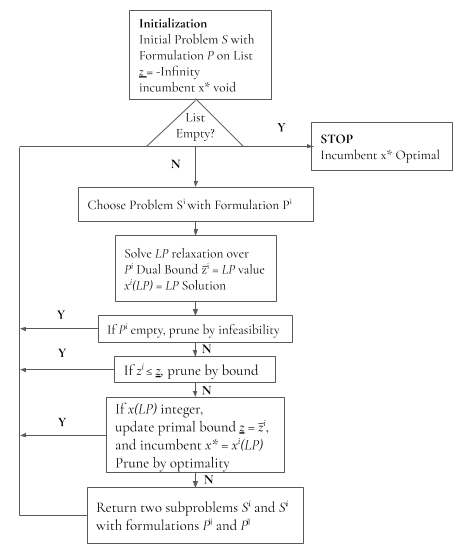
\includegraphics[scale=0.4]{flowchart.png}
\end{center}
\end{frame}

\begin{frame}
\frametitle{How are IPs Solved?}
\begin{itemize}
\item Gurobi will
    \begin{itemize}
    \item Run heuristics to try to find good feasible solutions earlier (improves upper bound)
    \item Add cutting planes to tighten LP relaxation (improves lower bound)
    \end{itemize}
\item You can help by
    \begin{itemize}
    \item Specifying an initial feasible solution using GRBVar attribute Start.
    \item Implement a callback to build heuristic solutions from relaxation solutions.
    \item Formulate your problem intelligently.
    \end{itemize}
\item Always set reasonable stopping criteria for IPs.
\end{itemize}
\end{frame}

\begin{frame}
\frametitle{Adding Constraints Can Improve Performance}
\begin{eqnarray}
\min_{x} && \sum_{i \in I} \sum_{j \in J} c_{ij} x_{ij} + \sum_{i \in I} f_i y_i \nonumber \\
\mbox{s.t.} && \sum_{i \in I} x_{ij} = d_j,\;\;j \in J \nonumber \\
&& \sum_{j \in J} x_{ij} \le u_i y_i,\;\;i \in I \nonumber \\
&& {\color{red} x_{ij} \le d_j y_i,\;\;i \in I,\;j \in J} \nonumber \\
&& x_{ij} \ge 0, \;\;i \in I,\;j \in J \nonumber \\
&& y_i \in \{0, 1\},\;\;i \in I \nonumber
\end{eqnarray}
Additional constraint is redundant, but can tighten the LP relaxation.
\end{frame}

\begin{frame}
\frametitle{Interdicting Nuclear Material Smuggling}
\begin{itemize}
\item Goal: Minimize probability of successful smuggling of nuclear material
\item Approach: Install radiation sensors at key locations
\item Question: How to select locations to achieve goal given limited resources?
\end{itemize}
\begin{center}
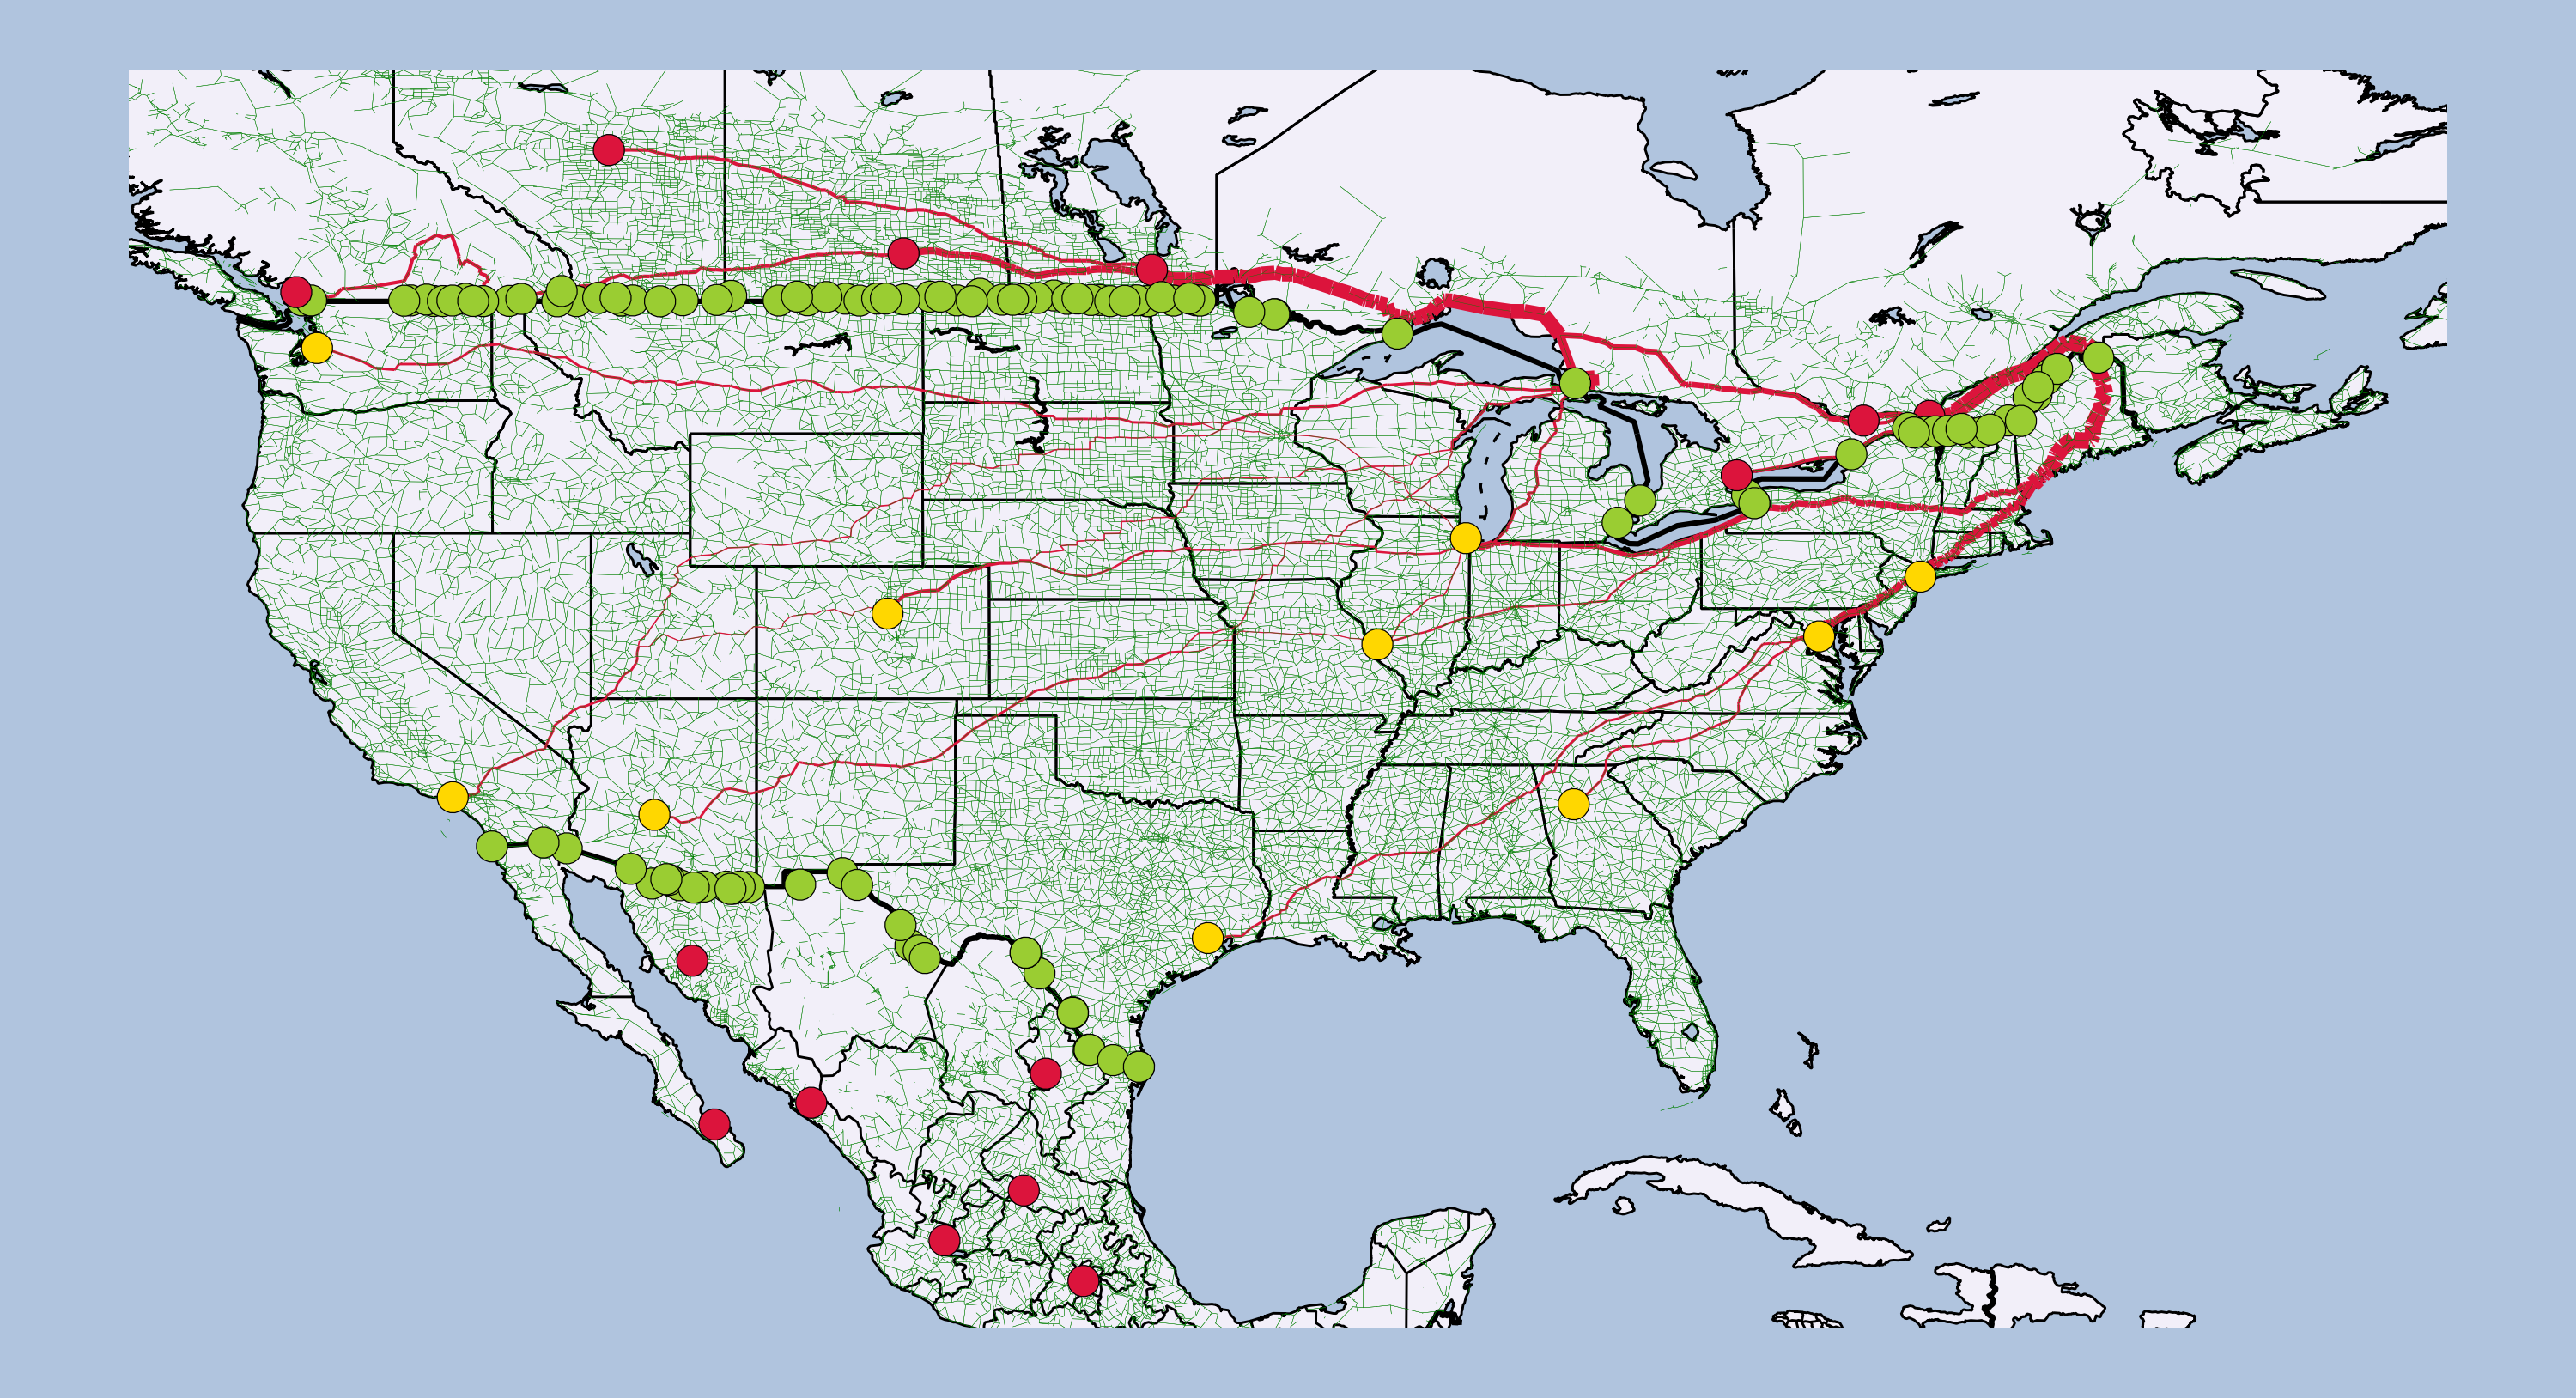
\includegraphics[scale=0.3]{checkpoints.png} \\
U.S. Land Border Crossings
\end{center}
\end{frame}
\begin{frame}
\frametitle{Interdicting Nuclear Material Smuggling}
\begin{center}
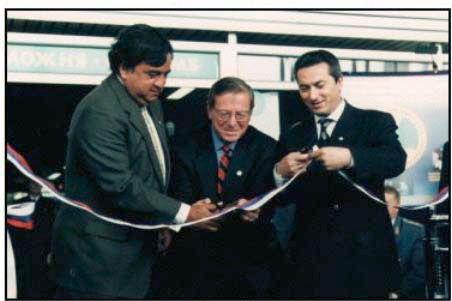
\includegraphics[scale=1]{ribbon_cutting.png} \\
Moscow's Sheremetyevo International Airport: September 1998
\end{center}
\end{frame}

\begin{frame}
\frametitle{Radiation Sensors in Sheremetyevo Airport}
\begin{center}
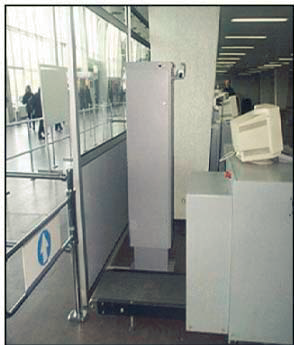
\includegraphics[scale=0.8]{detector1.png}
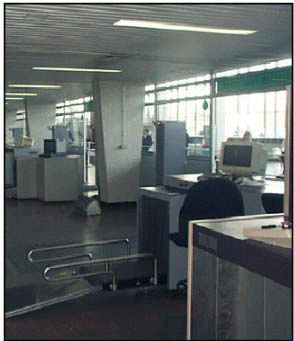
\includegraphics[scale=0.8]{detector2.png}
\end{center}
\end{frame}

\begin{frame}
\frametitle{SNIP: Stochastic Network Interdiction Problem}
Structure:
\begin{itemize}
\item Interdictor's decision: (First stage) Select locations to install sensors, subject to budget constraint
\item Random event: Smuggler's origin-destination pair is realized
\item Smuggler's decision: (Second stage) Select path from origin to destination to minimize probability of detection
\end{itemize}
Assumptions:
\begin{itemize}
\item Smuggler knows sensor locations, detection probabilities, chooses best path
\item Interdictor and smuggler ``see'' the same network
\end{itemize}
\end{frame}

\begin{frame}
\frametitle{One-Country Case}
\begin{itemize}
\item Potential smugglers indexed by $\omega \in \Omega$, with associated probability $p^\omega$
\item Checkpoints indexed by $k \in K$
\item Evasion probability $p_k^\omega$ if no sensor installed at checkpoint $k \in K$, 0 otherwise
\item Cost of installing sensor at checkpoint $c_k, k \in K$
\item Installation budget $b$
\end{itemize}
\begin{center}
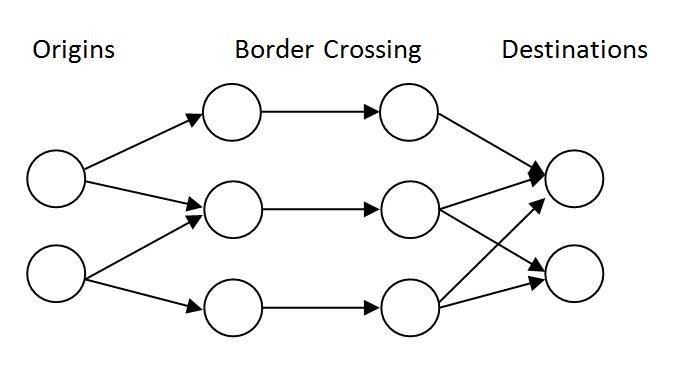
\includegraphics[scale=0.3]{one_country.jpg}
\end{center}
\end{frame}

\begin{frame}
\frametitle{Formulation}
Decision Variables:
\begin{itemize}
\item $x_k = 1$ if sensor installed at checkpoint $k$, 0 otherwise
\item $\theta^\omega$ : probability that smuggler $\omega$ evades detection, computed as $\theta^\omega = \max_{k \in K} p_k^\omega (1 - x_k)$
\end{itemize}
Model:
\begin{eqnarray}
\min_{x, \theta} && \sum_{\omega \in \Omega} p^\omega \theta^\omega \nonumber \\
\mbox{s.t.} && \theta^\omega \ge p_k^\omega - p_k^\omega x_k,\;\;k \in K,\;\omega \in \Omega \nonumber \\
&& \sum_{k \in K} c_k x_k \le b \nonumber \\
&& x_k \in \{0,1\},\;\;k \in K \nonumber
\end{eqnarray}
\end{frame}

\begin{frame}
\frametitle{Tightening the Formulation}
Consider $\theta^\omega \ge p_k^\omega - p_k^\omega x_k$, for a smuggler with $p_1^\omega = 1$, $p_2^\omega = 0.8$, $p_3^\omega = 0.6$, and $p_4^\omega = 0.4$.
\begin{eqnarray}
\theta^\omega &\ge& 1 - x_1 \nonumber \\
\theta^\omega &\ge& 0.8 - 0.8 x_2 \nonumber \\
\theta^\omega &\ge& 0.6 - 0.6 x_3 \nonumber \\
\theta^\omega &\ge& 0.4 - 0.4 x_4 \nonumber
\end{eqnarray}
\begin{itemize}
\item Role of $x_k$ in above is to make inequality non-binding if $x_k = 1$ \\
\item Making coefficients too large hurts solve time \\
\item Suppose budget constraint is $\sum_{k \in K} x_k \le 2$, can we make coefficients smaller?
\end{itemize}
\end{frame}

\begin{frame}
\frametitle{Big-M Coefficient Tuning}
\begin{itemize}
\item Rewrite $\theta^\omega \ge p_k^\omega - (p_k^\omega - \underline{\theta}^\omega) x_k$ where $\underline{\theta}^\omega$ is a lower bound on $\theta^\omega$.
\item Find $\underline{\theta}^\omega$ by allocating sensors to smuggler $\omega$'s best checkpoints
\item Wait-and-see bound
\end{itemize}
\end{frame}

\begin{frame}
\frametitle{Valid Inequalities}
Consider a smuggler with $p_1^\omega = 1$, $p_2^\omega = 0.8$, $p_3^\omega = 0.6$, and $p_4^\omega = 0.4$.
How much does smuggler evasion probability decrease as we interdict checkpoints?
\begin{equation}
\theta^\omega \ge 1 - 0.2 x_1 - 0.2 x_2 - 0.2 x_3 - 0.4 x_4 (1) \nonumber
\end{equation}
What if we ignore checkpoint 2?
\begin{equation}
\theta^\omega \ge 1 - 0.4 x_1 - 0.2 x_3 - 0.4 x_4 (2) \nonumber
\end{equation}
Both (1) and (2) are valid constraints to add. \\
Under what conditions is (1) stronger? \\
Under what conditions is (2) stronger?
\end{frame}

\begin{frame}
\frametitle{Valid Inequalities}
Consider smuggler $\omega$, and let $\{k_1, k_2, \ldots, k_n\}$ satisfy:
\begin{equation}
r_{k_1}^\omega \ge r_{k_2}^\omega \ge \cdots \ge r_{k_n}^\omega \nonumber
\end{equation}
Then
\begin{equation}
\theta^\omega \ge r_{k_1}^\omega - (r_{k_1}^\omega - r_{k_2}^\omega) x_{k_1} - \cdots - (r_{k_n}^\omega - 0) x_{k_l} \nonumber
\end{equation}
\begin{itemize}
\item The above ``step inequality'' can be written for any subset of checkpoints.
\item If $x_{k_{i+1}} > x_{k_i}$, then we should leave checkpoint $k_{i+1}$ out.
\item Exponentially many subsets, can't enumerate all possible step inequalities.
\end{itemize}
\end{frame}

\begin{frame}
\frametitle{Reformulation}
\begin{itemize}
\item Let $v_k^\omega = 1$ if smuggler $\omega$ traverses checkpoint $k$
\item Let $K_k^\omega = \{k' \in K : p_{k'}^\omega < p_k^\omega\}$ (i.e. checkpoints worse than $k$ from $\omega$'s perspective)
\item The following reformulation avoids big-M coefficients:
\end{itemize}
\begin{eqnarray}
\min_{x,v,\theta} && \sum_{\omega \in \Omega} p^\omega \theta^\omega \nonumber \\
\mbox{s.t.} && \theta^\omega = \sum_{k \in K} p_k^\omega v_k^\omega,\;\;\omega \in \Omega \nonumber \\
&& x_k \ge \sum_{k' \in K_k^\omega} v_{k'}^\omega,\;\;k \in K,\;\omega \in \Omega \nonumber \\
&& \sum_{k \in K} v_k^\omega = 1,\;\;\omega \in \Omega \nonumber \\
&& x_k \in \{0,1\},\;\;k \in K \nonumber \\
&& v_k^\omega \in \{0,1\},\;\;k \in K,\;\omega \in \Omega \nonumber
\end{eqnarray}
\end{frame}

\begin{frame}
\frametitle{Gurobi Parameters}
\begin{itemize}
\item Method : dual simplex, primal simplex, barrier
\item Presolve, PrePasses
\item Termination : IterationLimit, BarIterLimit, TimeLimit, NodeLimit, SolutionLimit, ...
\item Tolerances : FeasibilityTol, IntFeasTol, MIPGap, ...
\item MIP : Heuristics, MIPFocus, ImproveStartGap/Nodes/Time, ...
\item MIPCuts : Cuts, CutPasses, MIRCuts, ...
\item Some parameters are tied to a particular algorithm (i.e. barrier, simplex, MIP)
\item GRBEnv.set(parameter, value), Model.SetParam(parameter, value) in Python
\end{itemize}
\end{frame}

\begin{frame}
\frametitle{Metaparameters}
\begin{itemize}
\item Setting value of Cuts parameter will change level of aggressiveness for all cut types.
    \begin{itemize}
    \item Can be overridden for a particular type of cut by setting CliqueCuts, CoverCuts, etc.
    \end{itemize}
\item MIPFocus=1 (focus on feasiblity) sets CutPasses=5, Heuristics=0.2, and VarBranch=1
\item MIPFocus=2 (focus on optimality) sets Cuts=2, Presolve=2,
\end{itemize}
\end{frame}

\begin{frame}
\frametitle{Automatic Parameter Tuning}
\begin{itemize}
\item Through API via GRBModel.Tune()
\item Through command line via grbtune (grbtune [param=value] filename1 filname2 ...)
\item Goal: Vary parameters that matter (where is solve time being spent?)
\item Minimize runtime or minimize optimality gap
\item Parameters that control the parameter tuning tool:
    \begin{itemize}
    \item TuneTimeLimit
    \item TuneTrials
    \item TuneResults
    \item TuneOutput
    \item ResultFile
    \end{itemize}
\item Important parameters for difficult MIP models : MIPFocus, Presolve, Cuts, CutPasses, VarBranch, Method (if root relaxation difficult), Heuristics
\item Mean improvement from best settings over 423 models : 2.91X
\end{itemize}
\end{frame}

\begin{frame}
\frametitle{Callbacks}
\begin{itemize}
\item Create a subclass of GRBCallback and implement a callback() method
\item Call GRBModel.SetCallback(GRBCallback)
\item callback() method is called periodically during optimization
\item Query the protected member {\em where} to figure out where you are (PRESOLVE, MIPNODE, MIPSOL, etc.)
\item GRBCallback methods
    \begin{itemize}
    \item AddCut (if where is MIPNODE)
    \item AddLazy (if where is MIPNODE or MIPSOL)
    \item GetNodeRel (if where is MIPNODE and GRB.Callback.MIPNODE\_STATUS is GRB.OPTIMAL)
    \item GetSolution (if where is MIPSOL)
    \end{itemize}
\end{itemize}
\end{frame}

\begin{frame}
\frametitle{Custom Rounding Heuristics}
\begin{itemize}
\item If where == GRB.Callback.MIPNODE and GRB.Callback.MIPNODE\_STATUS == GRB.OPTIMAL
\item Call GRBCallback.GetNodeRel(vars) to get LP relaxation solution
\item Run heuristic
\item Call GRBCallback.SetSolution(vars, soln) to pass back the heuristic solution
\end{itemize}
\end{frame}

\end{document}
